\chapter{Literature Review}
\label{ch:background}

\section{A History of DeepFakes}

% \begin{itemize}
%     \item More detailed explanation of deepfakes
%     \item How are they generated
%     \begin{itemize}
%         \item GANs
%         \item assorted other AI shenanigans
%     \end{itemize}
% \end{itemize}

\subsection{Photo Manipulation}

Humans have been manipulating photographs since the 1860s when a composite of United States President Abraham Lincoln was composited onto fellow politician John Calhoun's body\cite{singh2018art} as shown in Figure \ref{fig:lincoln}. Photo tampering was then used throughout history as a way to shape opinions and beliefs of individuals by altering supposed ``evidence". As photography was still an entirely analogue process, editing a photo was significantly harder than it is today but nevertheless it still was done when deemed necessary. Another famous example is the removal of Nikolai Yezhov in 1940 from a 1937 photo (Figure \ref{fig:stalin-yezhov}) with Joseph Stalin after the ``Great Purge" in the Union of Soviet Socialist Republics.

\begin{figure}[H]
    \centering
    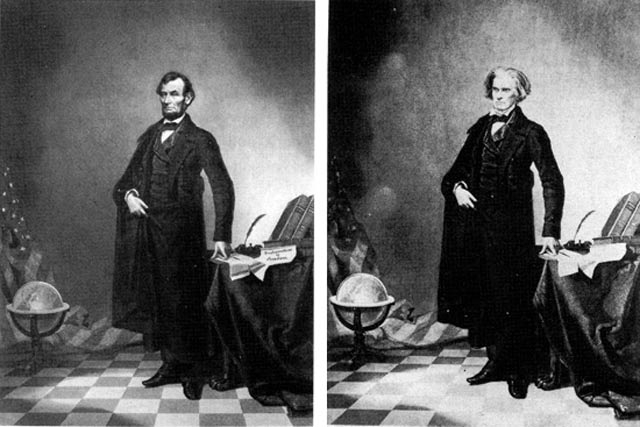
\includegraphics[width=0.5\linewidth]{dissertation//figures/lincoln1960.jpg}
    \caption{A spliced portrait of Abraham Lincoln (left) with the original (right)\cite{singh2018art}}
    \label{fig:lincoln}
\end{figure}

\begin{figure}[H]
    \centering
    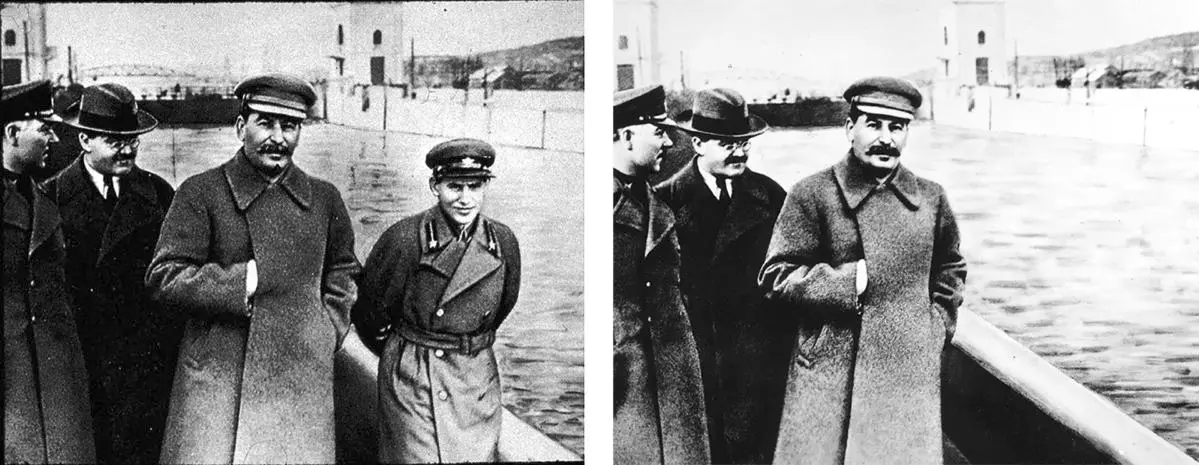
\includegraphics[width=0.5\linewidth]{dissertation//figures/stalin.png}
    \caption{A photo of Stalin and Yezhov which was subsequently edited to remove Yezhov}
    \label{fig:stalin-yezhov}
\end{figure}

With the advent of digital photography and computers, it photo manipulation became mainstream. Suddenly, images were not physical items but data stored on a computer which could be easily manipulated. Changes could be viewed instantly, reversed, and shared easily. Programs to edit images soon became possible such as Adobe Photoshop\footnote{\url{https://www.adobe.com/uk/products/photoshop.html}} and GIMP\footnote{\url{https://www.gimp.org/}}. Whilst these tools made photo editing cheap and accessible, they still required time, effort, and skill from humans in order to produce; an original image is also required for manipulation.

Computer Generated Imagery (CGI) is a technique primarily used in movies to add artificially augment a frame, often with complete novel additions. CGI was first used in the 1958 film ``Vertigo" and became widespread in the 1990s\cite{ozturk2023vicious}. In the present day, CGI is used in almost every blockbuster film to generate realistic images. In ``Rogue One: A Star Wars Story" the actor Peter Cushing digitally recreated after his death in 1994 to play Grand Moff Tarkin (Figure \ref{fig:tarkin}).While CGI requires large amounts of hardware, consumer image generation runs on much worse hardware but has equally progressed. Most modern social media apps contain a variety of beauty filters\cite{corcoran2014digital}. For example, a blur can be applied to reduce skin blemishes as shown by Figure \ref{fig:beauty-filter}. These are often less computationally expensive and so can run on smartphones, offering the ability to manipulate media to the masses, not just the technically-able and skilled.

\begin{figure}[H]
    \centering
    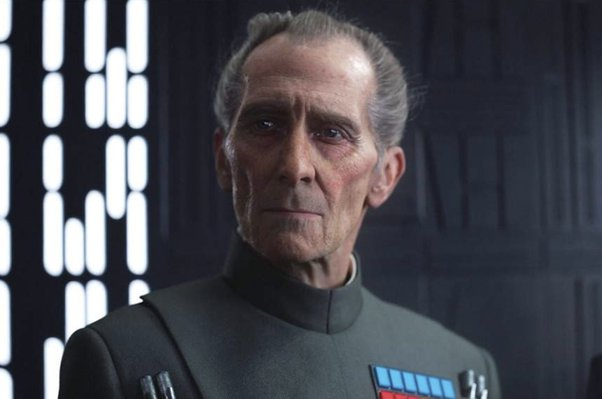
\includegraphics[width=0.5\linewidth]{dissertation//figures/grandmoff-tarkin.jpg}
    \caption{A digital recreation of Peter Cushing for the film ``Rogue One: A Star Wars Story"\cite{rogueone}}
    \label{fig:tarkin}
\end{figure}

\begin{figure}[H]
    \centering
    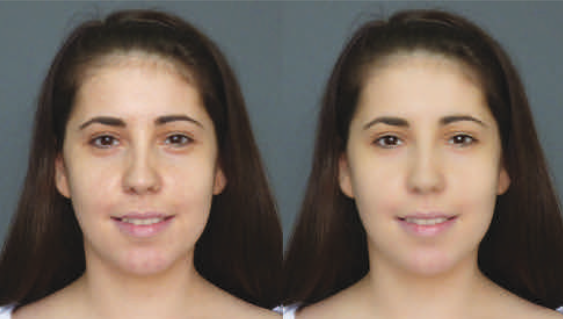
\includegraphics[width=0.5\linewidth]{dissertation//figures/blurring.png}
    \caption{An original image (left) blurred to remove skin blemishes (right)\cite{corcoran2014digital}}
    \label{fig:beauty-filter}
\end{figure}

\subsection{Artificial Intelligence for Manipulating Media}

\subsubsection{Convolutional Neural Networks}

DeepFakes are a type of AI known as neural networks. As described in Section \ref{sec:project-review}, neural networks are a subsection of AI designed of the structure of the human brain\cite{islam2019overview}. Traditional computation manipulates binary, whereas neural networks manipulate the connections between computational elements. Work on simulating the brain using mathematical functions began in 1920\cite{brush1967history}, 37 years before the academic formalisation of AI in 1957 at the Dartmouth Workshop\cite{crevier1993ai}. The field would remain relatively stagnant until the proposal of the Multi-Layer Perceptron (MLP) in 1958\cite{rosenblatt1958perceptron} and how it could ``learn" in 1967\cite{ivakhnenko1967cybernetics}.

Neural networks contain a collection of neurons organised into layers, each layer receives inputs from the neurons before (Figure \ref{fig:full-neural-network}). Each of the $n$ inputs has an associated weight ($w_i$) and value ($x_i$). Once the combined weights and an additional bias weight ($b$) exceed a determined threshold (usually 0) then the neuron fires with an output ($y$) determined by an activation function ($f(x)$). This is shown in Equation \ref{eq:neuron-activation} and Figure \ref{fig:neural-network}. The network shown in Figure \ref{fig:neural-network} has a 1 dimensional input, however MLPs can expand to an infinite number of dimensions.

\begin{equation}
\label{eq:neuron-activation}
    \begin{array}{c@{\hspace{2cm}}c}
        W = b+\displaystyle\sum_{i=1}^{n} w_ix_i  &
        y = \begin{cases}
            f(W) & \text{if } W \geq 0  \\
            0/-1 & \text{otherwise}
        \end{cases}
    \end{array}
\end{equation}

\begin{figure}[h]
    \centering
    \begin{subfigure}[t]{0.45\textwidth}
        \centering
        \begin{tikzpicture}
            % inputs
            \node[draw=none] (x1) at (-1,2) {\(x_1\)};
            \node[draw=none] (x2) at (-1,0) {\(x_2\)};
            \node[draw=none] (x3) at (-1,-2) {\(x_3\)};
            
            % nuron (split circle)
            \node[draw, circle, minimum size=1.8cm, thick] (neuron) at (3,0) {};
            \node at (2.5, 0) {\(\sum\)}; % Left side - Summation
            \node at (3.5, 0) {\(f\)}; % Right side - Activation
            \draw[thick] (neuron.south) -- (neuron.north); % dividing line
            
            % output
            \node[draw=none] (output) at (6,0) {\(y\)};
            \draw[->] (neuron.east) -- (output);
            
            % weights
            \draw[->] (x1) -- node[above] {\(w_1\)} (neuron.west);
            \draw[->] (x2) -- node[above] {\(w_2\)} (neuron.west);
            \draw[->] (x3) -- node[below] {\(w_3\)} (neuron.west);
            
            % bias
            \node[draw=none] (bias) at (3,-2.5) {\(b\)};
            \draw[->] (bias) -- (neuron.south);
        \end{tikzpicture}
        \subcaption{Structure of a single artificial neuron}
        \label{fig:neuron}
    \end{subfigure}
    \begin{subfigure}[t]{0.45\textwidth}
        \centering
        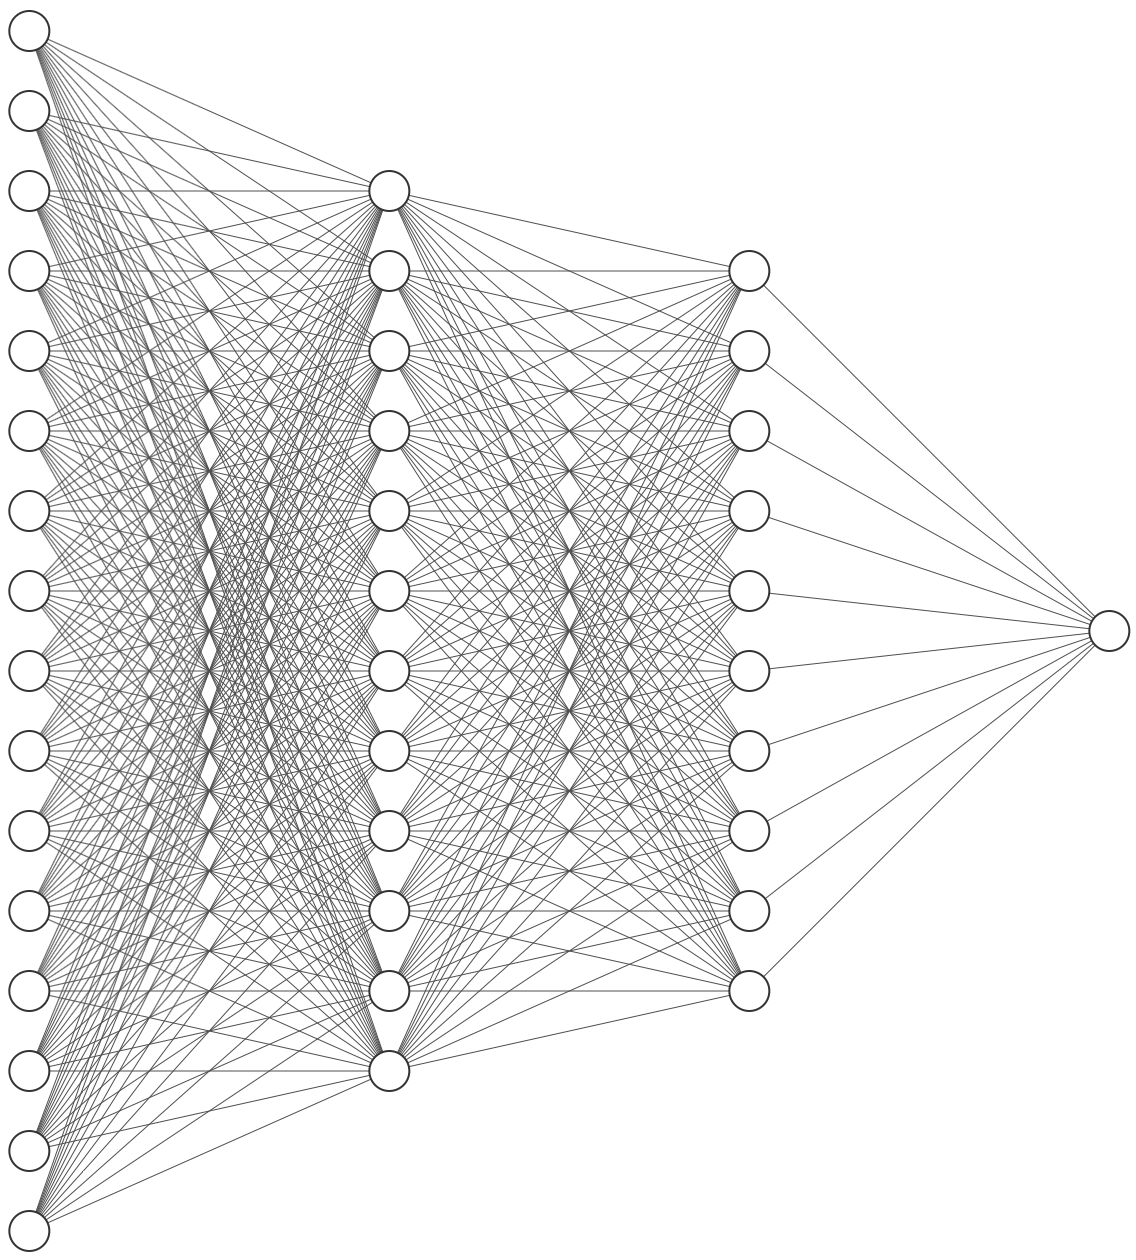
\includegraphics[width=0.75\textwidth]{dissertation//figures/generic-neural-diagram.png}
        \subcaption{A network of neurons split into layers}
        \label{fig:full-neural-network}
    \end{subfigure}
    \caption{A neural network}
    \label{fig:neural-network}
\end{figure}

Whilst MLPs are exceptionally powerful they can suffer from overfitting. Overfitting is where a machine learning model learns the training data, becoming exceptionally accurate in the training data but underperforms on any test data. With every neuron in an MLP layer being connected to all the neurons in the layers ahead and behind it, the network is prone to overfit\cite{o2015introduction}. A variety of methods can be employed to reduce overfitting, but the most common way removes connections from the network by reshaping the layers, this also has the attractive benefit of quicker computations as there are less weights to sum resulting in faster training and inference times. A number of methods to reduce connections have been proposed but the most successful are Convolutional Neural Networks (CNNs).

A CNN is a sequence of three layers: convolution layers, pooling layers, and a fully connected layer\cite{ibmconvolutional}. Each set of layers reduces the dimensions of the input, allowing each subsequent layer to take into account a larger portion of the image.

\begin{itemize}
    \item \textbf{Convolutional Layer}\\
    A Convolutional Layer is what a CNN lends its name to. It has two stages. The first stage is a filtering stage where a kernel (matrix) is passed over the input. The kernel is placed over the input and the dot product between the values in the kernel and the values in the input are calculated. This then becomes the output. The kernel is then shifted over by a fixed stride value to analyse another set of the input. This process is shown in Figure \ref{fig:filter}. The values (or weights) of each filter remain constant as it moves across the image, there can also be many filters, increasing the dimension of an input. These values are what are learned by this layer, by reducing the values to be trained to the size of the filter, this significantly speeds up the training process. Often some form of activation layer will be included to process the output array, more often than not, this uses the Rectified Linear Unit (ReLU) function, to limit outputs to strictly positive in order to introduce linerarity and prevent the vanishing gradient problem (a hindrance to learning)\cite{ibmconvolutional}.
    \begin{figure}[h]
        \centering
        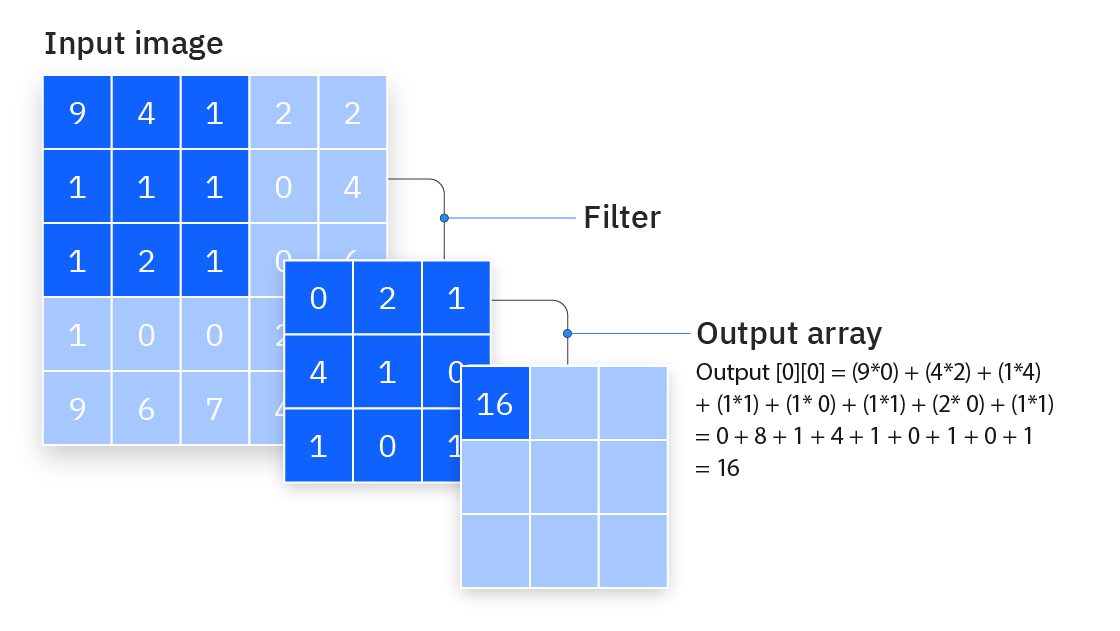
\includegraphics[width=0.5\linewidth]{dissertation//figures/cnn-filter.png}
        \caption{A diagram showing the action of a $3 \times 3$ filter\cite{ibmconvolutional}}
        \label{fig:filter}
    \end{figure}

    \item \textbf{Pooling Layer}\\
    The Pooling Layer is similar downsampling layer to the convolution layer but with no learnable parameters. Instead of a weighted kernel an aggregation function pools multiple values into a single one\cite{o2015introduction}. Any function could be used but the most common ones are: max pooling where the maximum value under the kernel is selected; or average pooling where the average of all the values is chosen. Pooling layers further reduce the numbers of learning parameters: reducing the tendency for overfitting, the model complexity, and computation time\cite{ibmconvolutional}.

    \item \textbf{Dense Layer}\\
    To produce an output that is usable a final dense layer is needed to convert the output of the previous layers into a desired shape. This is an fully connected MLP network.
\end{itemize}

A sequence of these layers are then combined to produce a network. The exact sequence and order is defined by the network architect and depends on the level of quality of output they want. More layers means a higher probable accuracy but incurs increased computation and tendency overfit. Further techniques exist to enhance CNNs such as skip connections which results in the outputs of layers to ``skip" forward layers and act as the input for layers further down the network. An example of a CNN to classify images is shown in Figure \ref{fig:sample-cnn}:

\begin{figure}[H]
    \centering
    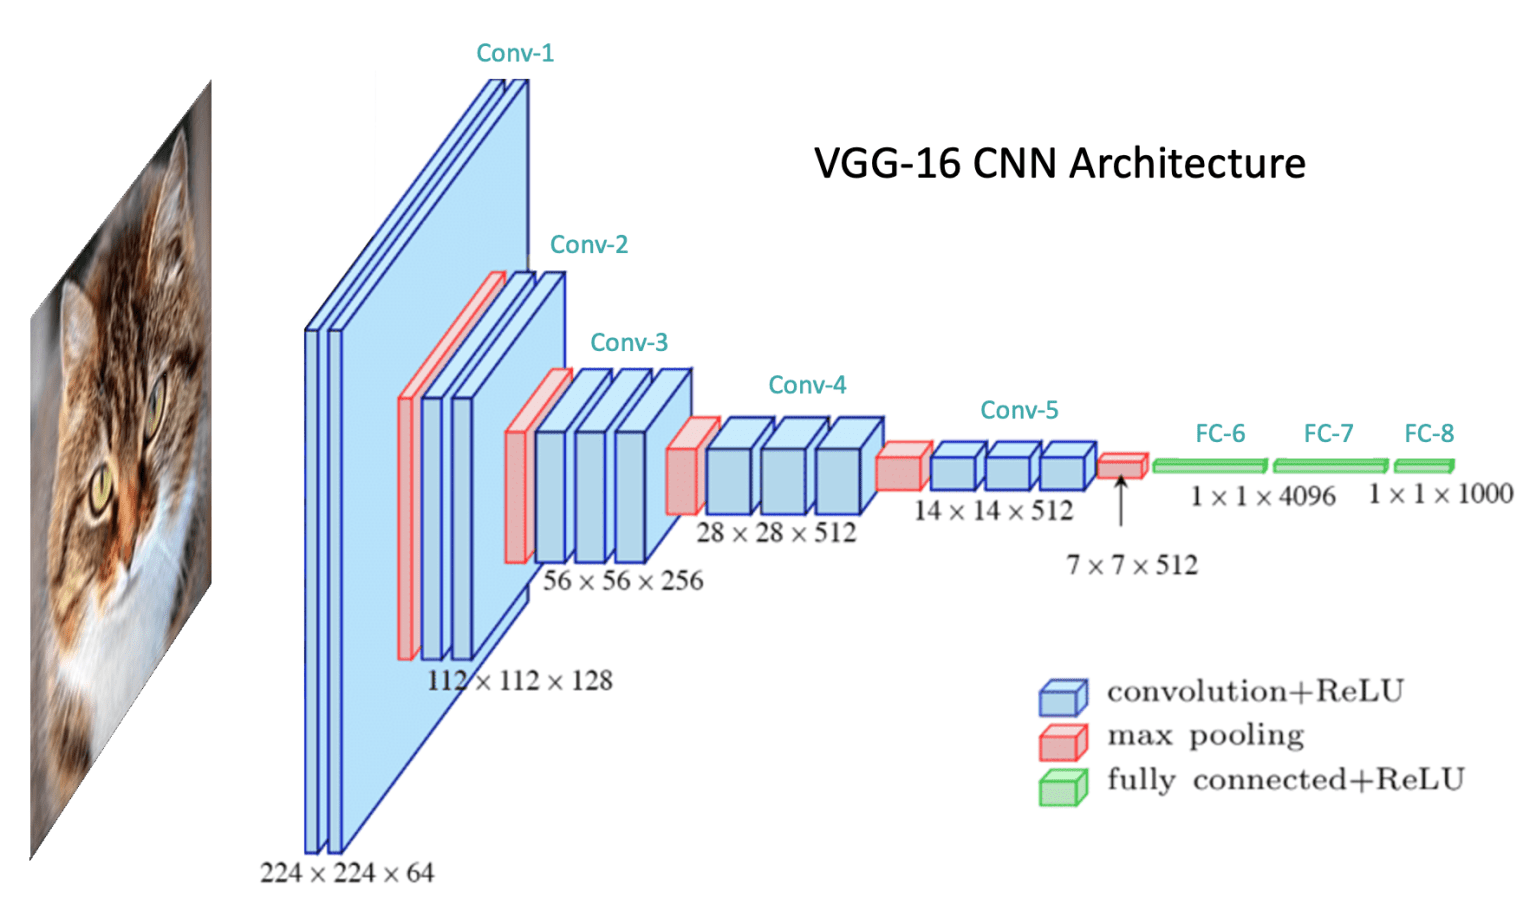
\includegraphics[width=0.5\linewidth]{dissertation//figures/sample-cnn.png}
    \caption{A sample CNN network\cite{kromydas2023convolutional}}
    \label{fig:sample-cnn}
\end{figure}

{\huge add stuff to train here (stochastic graident descent and adam)}

\section{DeepFake Detection}

\subsection{Traditional Detection Methods}

\begin{itemize}
    \item Backbones
    \begin{itemize}
        \item ResNet, VGG19....
        \item Head added for final classification
        \item Often trained on imagenet (transfer learning)
    \end{itemize}
\end{itemize}

\subsection{Blink-Based Detection Methods}

\begin{itemize}
    \item Human's blink in a periodic and predictable manner
    \item DeepFakes struggle with temporal stuff
    \item Eye Aspect Ratio
    \item DeepVision
    \item Ictu Oculi
    \item see progress report for evaluation and other stuff
\end{itemize}

\section{Adversarial Noise}

\begin{itemize}
    \item Additive noise can cause misclassification
    \item Adversarial Perturbations
    \item FakeRetouch
    \item Again see progress report
\end{itemize}

\section{Datasets}

\begin{itemize}
    \item Wide variety of deepfake datasets (they be chonky)
    \item most require request for access
    \item DFDC is a pain
\end{itemize}